{\color{gray}Consider a relational database for information related to cheese products, with the following tables:

\tab CHEESE( \underline{cheeseID}, type, producer, calories, proteins )

\tab REGION( \underline{regionID}, name, country)

\tab PRODUCTION ( \underline{productionID}, cheeseID, season, amount )

\tab PROVENANCE ( \underline{productionID, regionID} )

Assume that the following three stored procedures can run concurrently in a given application that is supported by the relational database:
\begin{enumerate}

	\item \textbf{insert\_cheese}: creates new records in the CHEESE table, for new cheeses that are produced. This procedure uses only the CHEESE table.

	\item \textbf{update\_production}: inserts new records, or modifies existing PRODUCTION and PROVENANCE records. This procedure writes to the PRODUCTION and PROVENANCE tables, updates the tuples in the PROVENANCE table, and may be reading from the REGION and CHEESE tables.

	\item \textbf{delete\_region}: deletes a given region from the REGION table.

\end{enumerate}
}

\subsection{}
{\color{gray}Give a scenario that leads to a possible dirty read in the concurrent execution of operations from this group of stored procedures, or explain why a dirty read cannot happen in this group of stored procedures.}

Consider two transactions both using \textbf{update\_production} stored procedure over the same PRODUCTION tuples.

\begin{figure}[H]
	\centering
	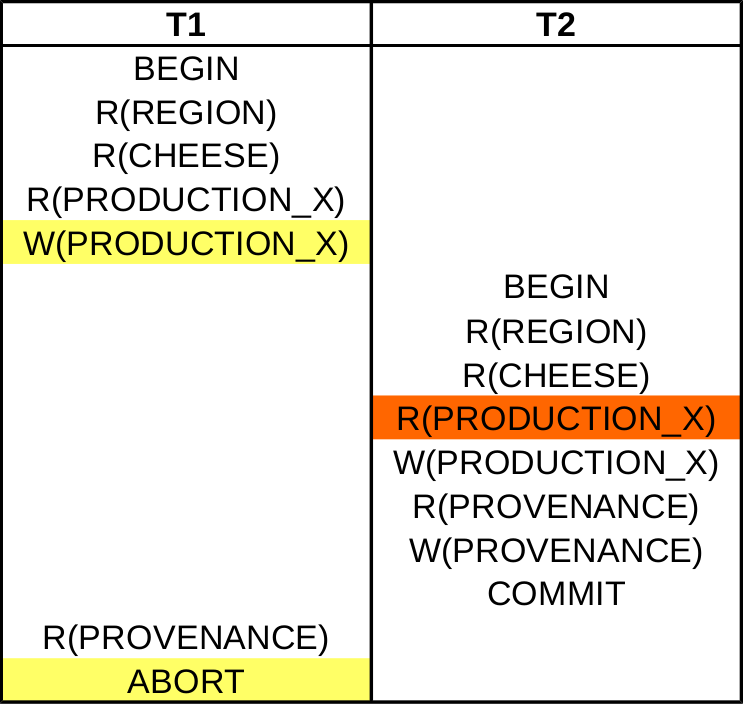
\includegraphics[width=0.35\textwidth]{dirty_read.png}
	\caption{An example of dirty read}
\end{figure}

T2 commits and T1 aborts after, rolling back its changes, the PRODUCTION tuples that T2 read from T1 are dirty reads because they reflect changes of an aborted transaction (T1). 

\subsection{}
{\color{gray}Give a scenario that leads to a possible non-repeatable read in the concurrent execution of operations from this group of stored procedures, or explain why a non-repeatable read cannot happen in this group of stored procedures.}

Consider that transaction one executes two \textbf{update\_production} stored procedures over the same REGION tuple, the second transaction deletes this REGION tuple.

\begin{figure}[H]
	\centering
	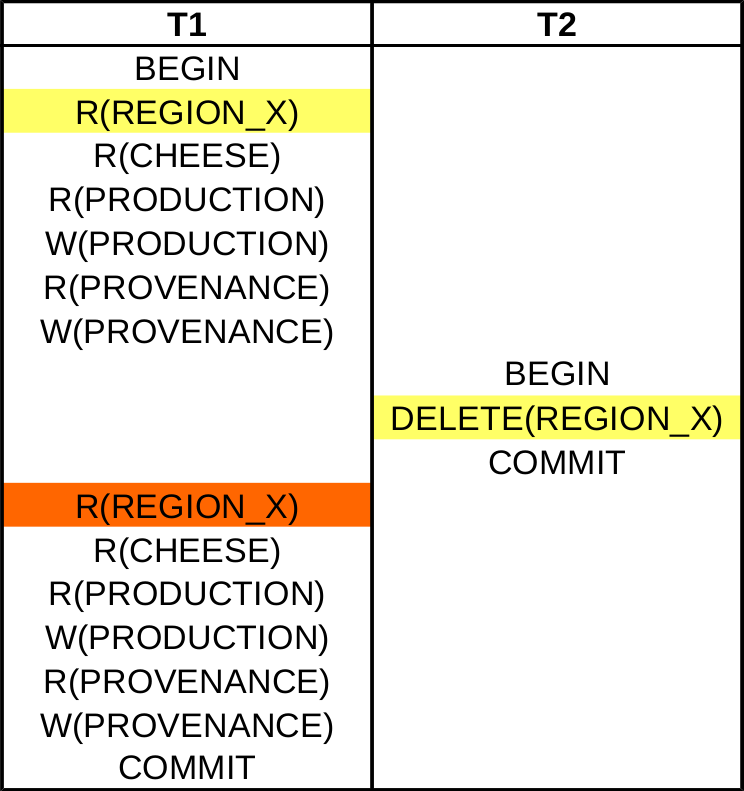
\includegraphics[width=0.35\textwidth]{unrepeatable_read.png}
	\caption{An example a non-repeatable read}
\end{figure}

The second time the REGION tuple is read, it doesn't exists, leading to  a non-repeatable read.

\subsection{}
{\color{gray}Give an example of a possible overwriting of uncommitted data in the concurrent execution of operations from this group of stored procedures, or explain why a phantom read cannot happen in this group of stored procedures.}

Consider two transactions both using \textbf{update\_production} stored procedure over the same PRODUCTION tuples.

\begin{figure}[H]
	\centering
	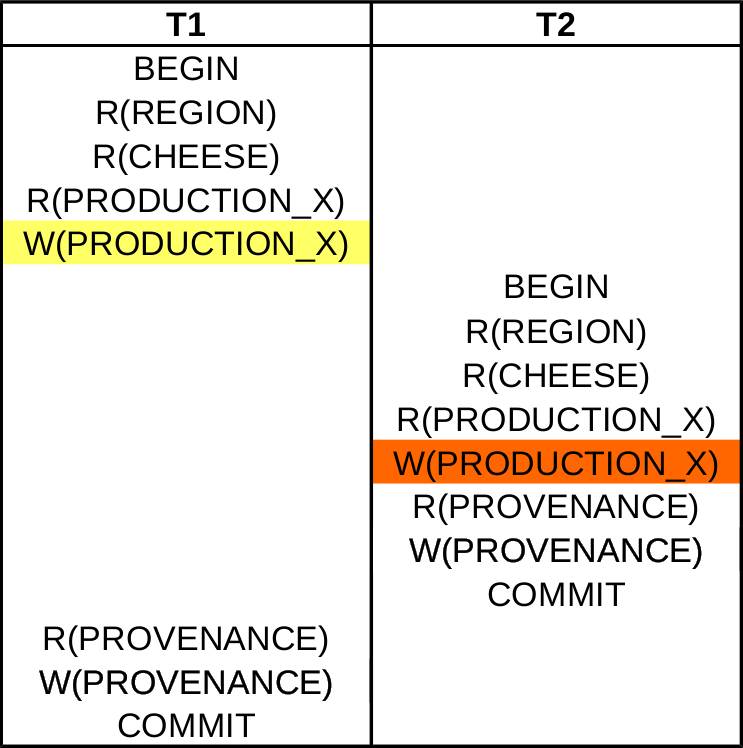
\includegraphics[width=0.35\textwidth]{overwrite_uncommit.png}
	\caption{An example overwriting of uncommitted data}
\end{figure}

T2 commits and T1 PRODUCTION tuple value is lost. 

\subsection{}
{\color{gray}Indicate what transaction isolation level would you use for executing each of the three procedures above, and why? For each procedure you should use the least restricted transaction isolation level that ensures correctness.}


\begin{enumerate}

	\item \textbf{insert\_cheese}: read uncommited, because one either serializable or not, if two transactions insert the same cheese, one of them must fail with a violation of the primary key constraint.

	\item \textbf{update\_production}: repeatable read, if a read over the same PRODUCTION or PROVENANCE tuples occurs, the second transaction should wait for the first to commit.

	\item \textbf{delete\_region}: read commited, because if an update\_production is happening the delete should wait for it to commit (update\_production has read a region)

\end{enumerate}
